\graphicspath{{figures/appendix-inflow/}}

\chapter{各激发态能级的主要产生过程}
\label{appendix:main-inflow}

这里给出与第 \ref{sec:main-inflow} 节不同的其他 $n_{\rm e}$ 与 $T_{\rm e}$ 条件下,各激发态能级的主要产生过程粒子流图,单位:${\rm cm}^{-3}{\rm s}^{-1}$。其中,虚线箭头为自发辐射跃迁过程,实线箭头为碰撞跃迁过程。
\begin{center}
\fbox{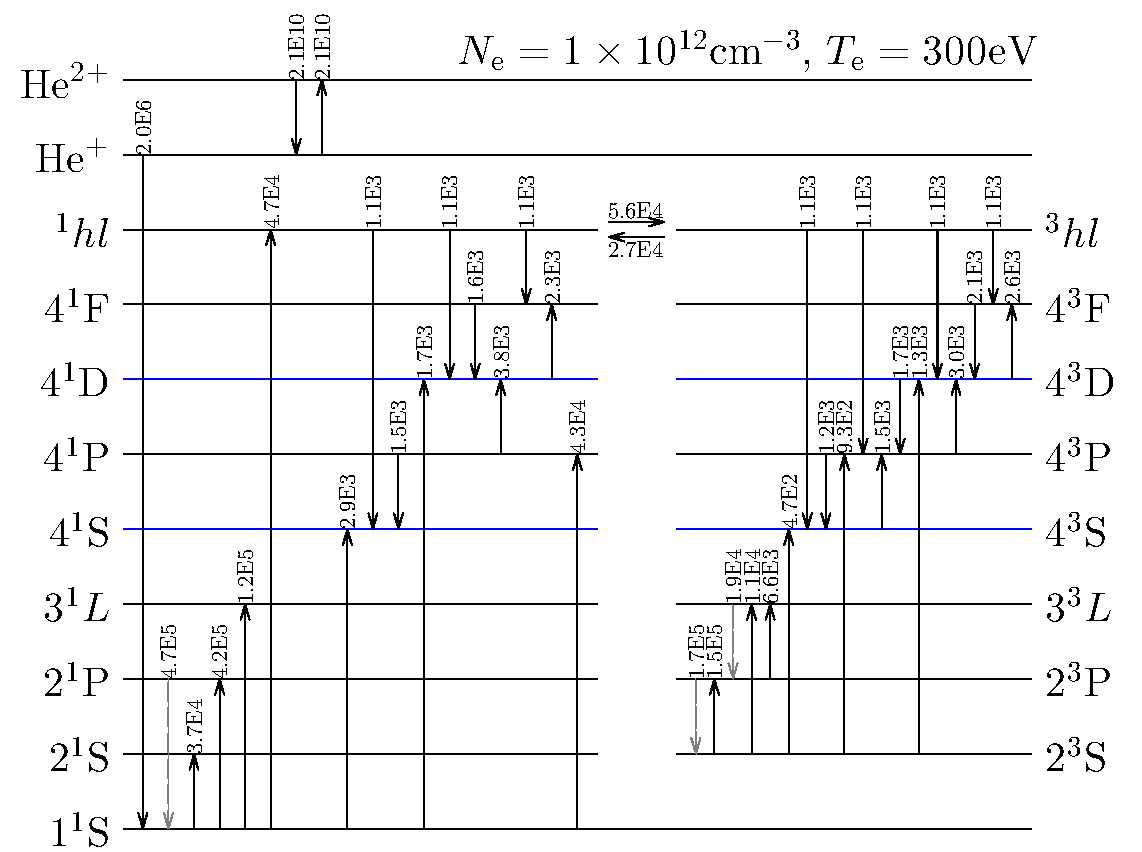
\includegraphics[width=0.8\textwidth]{Ne1E12_Te300_1e7cm-3s-1.pdf}}\\
\vspace{2em}
\fbox{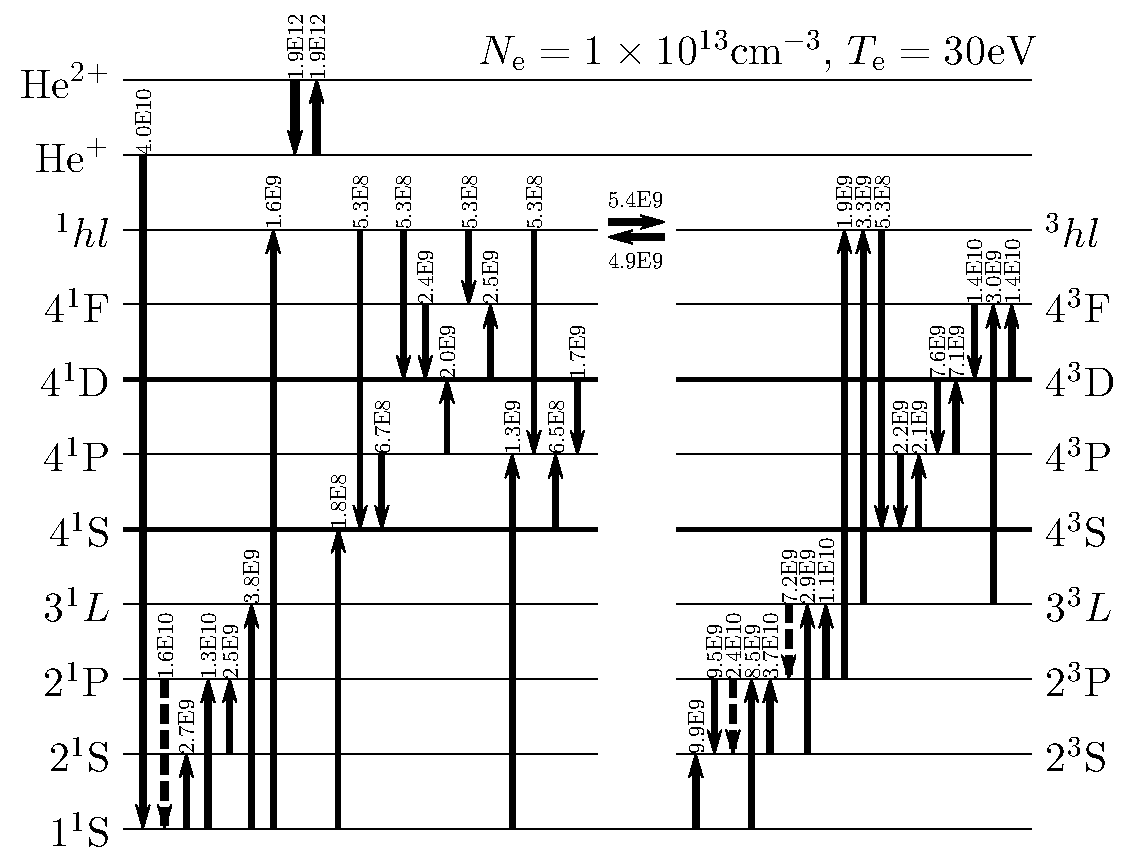
\includegraphics[width=0.8\textwidth]{Ne1E13_Te30_1e7cm-3s-1.pdf}}\\
\vspace{2em}
\fbox{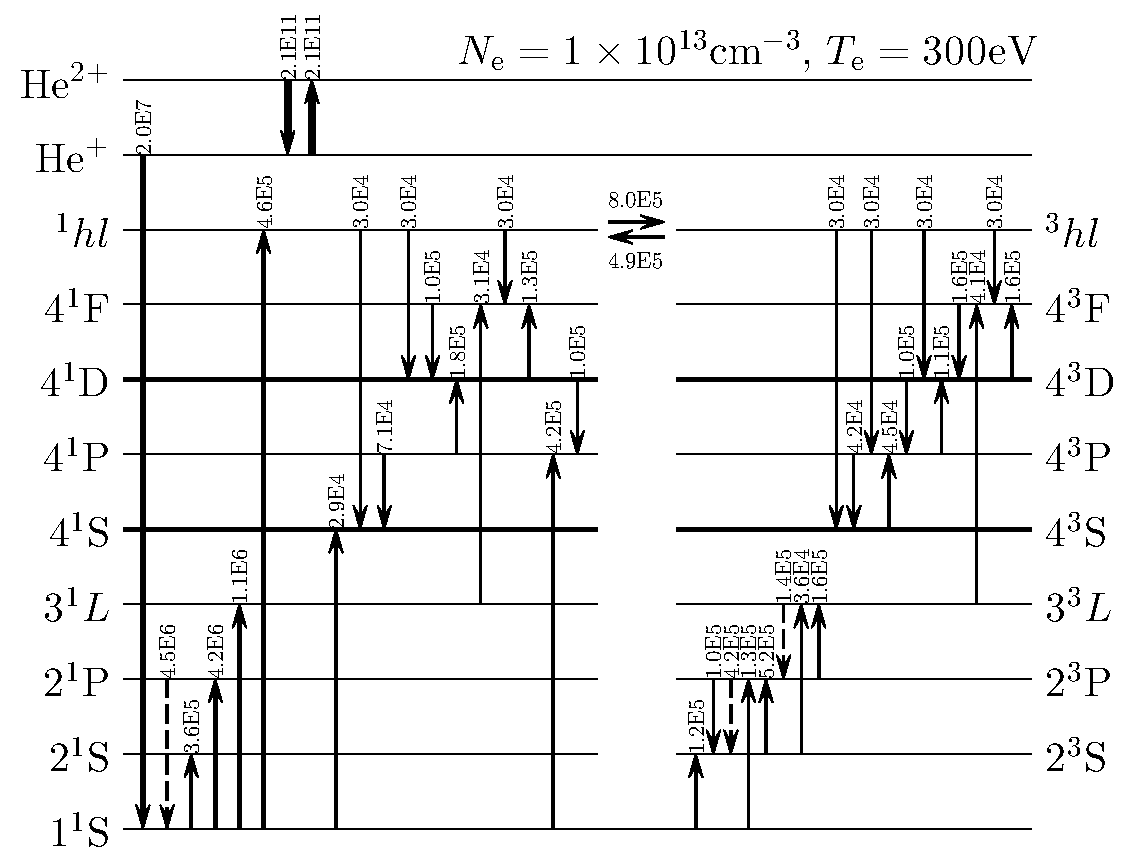
\includegraphics[width=0.8\textwidth]{Ne1E13_Te300_1e7cm-3s-1.pdf}}
\end{center} 